\documentclass[12pt]{article}
\usepackage{latexsym,amssymb,amsmath} % for \Box, \mathbb, split, etc.
% \usepackage[]{showkeys} % shows label names
\usepackage{cite} % sorts citation numbers appropriately
\usepackage{path}
\usepackage{url}
\usepackage{verbatim}
\usepackage{graphicx}
\usepackage{array}
\usepackage{multirow}

% horizontal margins: 1.0 + 6.5 + 1.0 = 8.5
\setlength{\oddsidemargin}{0.0in}
\setlength{\textwidth}{6.5in}
% vertical margins: 1.0 + 9.0 + 1.0 = 11.0
\setlength{\topmargin}{0.0in}
\setlength{\headheight}{12pt}
\setlength{\headsep}{13pt}
\setlength{\textheight}{625pt}
\setlength{\footskip}{24pt}

\renewcommand{\textfraction}{0.10}
\renewcommand{\topfraction}{0.85}
\renewcommand{\bottomfraction}{0.85}
\renewcommand{\floatpagefraction}{0.90}
\usepackage{graphicx}
\usepackage{wrapfig}
\usepackage{lscape}
\usepackage{rotating}
\usepackage{epstopdf}
\makeatletter
\setlength{\arraycolsep}{2\p@} % make spaces around "=" in eqnarray smaller
\makeatother

% change equation, table, figure numbers to be counted inside a section:
\numberwithin{equation}{section}
\numberwithin{table}{section}
\numberwithin{figure}{section}

% begin of personal macros
\newcommand{\half}{{\textstyle \frac{1}{2}}}
\newcommand{\eps}{\varepsilon}
\newcommand{\myth}{\vartheta}
\newcommand{\myphi}{\varphi}
\usepackage[utf8]{inputenc}

% Default fixed font does not support bold face
\DeclareFixedFont{\ttb}{T1}{txtt}{bx}{n}{8} % for bold
\DeclareFixedFont{\ttm}{T1}{txtt}{m}{n}{8}  % for normal

% Custom colors
\usepackage{color}
\definecolor{deepblue}{rgb}{0,0,0.5}
\definecolor{deepred}{rgb}{0.6,0,0}
\definecolor{deepgreen}{rgb}{0,0.5,0}
\definecolor{backcolour}{rgb}{0.96,0.96,0.96}

\usepackage{listings}

% cpp style for highlighting
\newcommand\cppstyle{\lstset{
		language=C++,
        basicstyle=\tiny\ttfamily,
		keywordstyle=\color{blue}\ttfamily,
		stringstyle=\color{red}\ttfamily,
		commentstyle=\color{green}\ttfamily,
		morecomment=[l][\color{magenta}]{\#},
		frame=tb,                         % Any extra options here
showstringspaces=false,            % 
backgroundcolor=\color{backcolour}
}}


% cpp environment
\lstnewenvironment{cpp}[1][]
{
	\cppstyle
	\lstset{#1}
}
{}

% cpp for external files
\newcommand\cppexternal[2][]{{
		\cppstyle
		\lstinputlisting[#1]{#2}}}

% cpp for inline
\newcommand\cppinline[1]{{\cppstyle\lstinline!#1!}}

\newcommand{\IN}{\mathbb{N}}
\newcommand{\IZ}{\mathbb{Z}}
\newcommand{\IQ}{\mathbb{Q}}
\newcommand{\IR}{\mathbb{R}}
\newcommand{\IC}{\mathbb{C}}
\newcommand{\Real}[1]{\mathrm{Re}\left({#1}\right)}
\newcommand{\Imag}[1]{\mathrm{Im}\left({#1}\right)}
\usepackage{booktabs}
\usepackage{caption}
\usepackage{float}
\usepackage{titlesec}
\usepackage{capt-of}
%dashed line
\usepackage{array}
\usepackage{arydshln}
\setlength\dashlinedash{0.2pt}
\setlength\dashlinegap{1.5pt}
\setlength\arrayrulewidth{0.3pt}

%Widows & Orphans & Penalties

\widowpenalty500
\clubpenalty500
\clubpenalty=9996
\exhyphenpenalty=50 %for line-breaking at an explicit hyphen
\brokenpenalty=4991
\predisplaypenalty=10000
\postdisplaypenalty=1549
\displaywidowpenalty=1602
\floatingpenalty = 20000
\usepackage[T1]{fontenc}
\usepackage{fontspec}
\setmainfont[Scale=0.85, Ligatures={Required,Common,Contextual,TeX}]{TeX Gyre Schola} % Incredible font inside latex


\newcommand{\norm}[2]{\|{#1}\|_{{}_{#2}}}
\newcommand{\abs}[1]{\left|{#1}\right|}
\newcommand{\ip}[2]{\left\langle {#1}, {#2} \right\rangle}
\newcommand{\der}[2]{\frac{\partial {#1}}{\partial {#2}}}
\newcommand{\dder}[2]{\frac{\partial^2 {#1}}{\partial {#2}^2}}
\usepackage{enumitem}
\newcommand{\nn}{\mathbf{n}}
\newcommand{\xx}{\mathbf{x}}
\newcommand{\uu}{\mathbf{u}}
\usepackage{tikz}
\usetikzlibrary{arrows}
\usetikzlibrary{positioning}
\usepackage{titlesec}
\newcommand{\junk}[1]{{}}
\usepackage{sectsty}
\usepackage{xcolor}

\newcommand\MyBox[2]{
	\fbox{\lower0.75cm
		\vbox to 1.7cm{\vfil
			\hbox to 1.7cm{\hfil\parbox{1.4cm}{#1\\#2}\hfil}
			\vfil}%
	}%
}

\makeatletter
\renewcommand*\env@matrix[1][\arraystretch]{%
	\edef\arraystretch{#1}%
	\hskip -\arraycolsep
	\let\@ifnextchar\new@ifnextchar
	\array{*\c@MaxMatrixCols c}}
\makeatother

\makeatletter
\renewcommand*\env@matrix[1][*\c@MaxMatrixCols c]{%
	\hskip -\arraycolsep
	\let\@ifnextchar\new@ifnextchar
	\array{#1}}
\makeatother

\definecolor{darkblue}{rgb}{0,0,0.4}
\usepackage[colorlinks = true,
linkcolor = darkblue,
urlcolor  = darkblue,
citecolor = darkblue,
anchorcolor = darkblue]{hyperref}
% set two lengths for the includegraphics commands used to import the plots:
\newlength{\fwtwo} \setlength{\fwtwo}{0.45\textwidth}
% end of personal macros

\begin{document}
\DeclareGraphicsExtensions{.jpg}

\begin{center}
\textsc{\Huge Multi-core Programming} \\[2pt]
	\textsc{\Large Assignment 6}\\
	\vspace{0.5cm}
  Ali Gholami \\[6pt]
  Department of Computer Engineering \& Information Technology\\
  Amirkabir University of Technology  \\[6pt]
  \def\UrlFont{\em}
  \url{https://aligholamee.github.io}\\
\href{mailto:aligholami7596@gmail.com}{\textit{aligholami7596@gmail.com}}
\end{center}

\begin{abstract}
The main purpose of this report is to analyze techniques to optimize the performance of a CUDA Kernel for \textit{reduction} task. Reduction is to find the sum of elements of an input array. We'll start with a naive implementation and we improve the performance in latter kernels. This can be done by removing bank conflict of warps while accessing the shared memory or removing the branch divergence by purposing new perspectives of thinking about conditional statements.
\end{abstract} 

\subparagraph{Keywords.} \textit{Reduction Strategies, Bank Conflict, Idle Threads, Loop Unrolling, Branch Divergence, Performance Optimization.}

\section{Memory Bandwidth Analysis}
\textit{Reduction} is a memory bounded task. Since the operational intensity is limited to 1 (we'll improve that in upcoming kernels), the memory bandwidth needs to be as high as possible to hide the effect of slow data access on performance. In this section, we'll compute the memory bandwidth for a \textit{Nvidia 850m GTX}. According to the information extracted by \textit{GPU-Z}, memory has a 128 bit interface with a clock of 1001 Mhz which yields in a bandwidth of 32 GB/s which is the peak bandwidth of this GPU.

\section{A Naive Reduction}
As an introduction to the reduction strategies, we'll provide a naive implementation of the reduction technique. This implementation suffers from:
\begin{itemize}
	\item Branch Divergence
\end{itemize}
at its core logic. Note that this implementation simply does a \textit{tree-based} reduction based on the copied input on to the shared memory. If the resulting array's size is greater than what a block can handle, it launches another kernel to compute the final results. The \textbf{problem} with this logic is that, 1 out of 2 threads will be diverged in the following \textit{conditional-check}:
\begin{cpp}
	// Tree based reduction
	for (unsigned int d = 1; d < blockDim.x; d *= 2) {
		if (tId % (2 * d) == 0)
			if (tId + d < blockDim.x)
				sData[tId] += sData[tId + d];
		
		__syncthreads();
	}
\end{cpp}
\subsubsection*{Removed Branch Divergence}
The code in the previous section can be improved by doing an \textit{index-based} condition as follows:
\begin{cpp}
	// Tree based reduction
	for (unsigned int d = 1; d < blockDim.x; d *= 2) {
		int index = 2 * d * tId;
		
		if (index < blockDim.x)
			if (index + d < blockDim.x)
				sData[index] += sData[index + d];
		
		__syncthreads();
	}
\end{cpp}
This improvement introduces a new problem; \textit{Shared Memory Bank Conflicts}. Data in shared memory is stored at \textit{words}. Each word is a 4 byte data type that is assigned to a shared memory bank of the same index. If we assume that there are total number of 32 banks of shared memory in each thread block, words 0 to 31 are assigned to banks 0 to 31. Respectively, words 32 to 63 are assigned to banks 0 to 31 an so on. If threads of a single warp request banks with the \textit{same index}, their request has to be processed \textit{sequentially}. This can be a great bottleneck which results in a \textit{memory-bound} kernel.
\subsubsection*{Removed Bank Conflicts}
This problem can be solved using \textit{sequential addressing}. If all threads in a warp request sequential shared memory indexes, the final bank conflict is at least as possible. This can be done using a reversed tree based reduction:
\begin{cpp}
	// Tree based reduction
	for (unsigned int d = blockDim.x/2; d > 1; d >>= 1) {
		if (tId < d)
			if (tId + d < blockDim.x)
				sData[tId] += sData[tId + d];		// Sequential Addressing
		
		__syncthreads();
	}
\end{cpp}
As it illustrates, in the first iteration, there are \textit{blockdim.x / 2} idle threads. This can turn into a huge waste. To solve the issue on the first iteration we'll provide the next improvement.
\subsubsection*{Solved Idle Threads Problem}
This approach uses the initial \textit{identification} section to perform an addition (reduction) when each thread finds its own global id.
\begin{cpp}
	// Identification
	unsigned int tId = threadIdx.x;
	unsigned int i = blockIdx.x * (2 * blockDim.x) + threadIdx.x;
	
	// Tree based reduction
	for (unsigned int d = blockDim.x / 2; d > 1; d >>= 1) {
		if (tId < d)
			if (tId + d < blockDim.x)
				sData[tId] += sData[tId + d];		// Sequential Addressing
		
		__syncthreads();
	}
\end{cpp}
It is obvious that when the size of the \textit{d} is less than 32, everything is being done within a warp. Thus we can remove \textit{\_\_syncthreads()} which saves a lot of time. The procedure of converting for loop iterations to instructions that aren't relying on each other based on a for loop, is called \textit{loop unrolling}. This increases the operational intensity of the kernel. Also, \textit{tId < d} can be removed while \textit{d} is less than 32.
\subsubsection*{Unrolled Warps}
\begin{cpp}
	// Identification
	unsigned int tId = threadIdx.x;
	unsigned int i = blockIdx.x * (2 * blockDim.x) + threadIdx.x;
	
	// Initialize
	sData[tId] = 0;
	
	__syncthreads();
	
	// Fill up the shared memory
	if (tId < blockDim.x) {
		sData[tId] = g_inData[i] + g_inData[i + blockDim.x];
	}
	
	__syncthreads();
	
	// Tree based reduction
	for (unsigned int d = blockDim.x / 2; d > 32; d >>= 1) {
		if (tId < d)
			if (tId + d < blockDim.x)
				sData[tId] += sData[tId + d];		// Sequential Addressing
		
		__syncthreads();
	}
	
	// Unrolled warps
	if (tId < 32) {
		sData[tId] += sData[tId + 32];
		sData[tId] += sData[tId + 16];
		sData[tId] += sData[tId + 8];
		sData[tId] += sData[tId + 4];
		sData[tId] += sData[tId + 2];
		sData[tId] += sData[tId + 1];
	}
\end{cpp}

\subsection*{Performance Analysis}
Performance results for 1B element reduction is given in table 1.1. For a larger input array, GPU performs drastically better. Comparing the serial timings with computation times is not fair. It is fair to compare total time for GPU with serial time. In this case the best speed up is \textit{1.43} compared to serial time. This is what happens in practice. Best computation speed up is \textit{16} which is obtained using the last kernel.
\begin{figure}[!h]\centering
	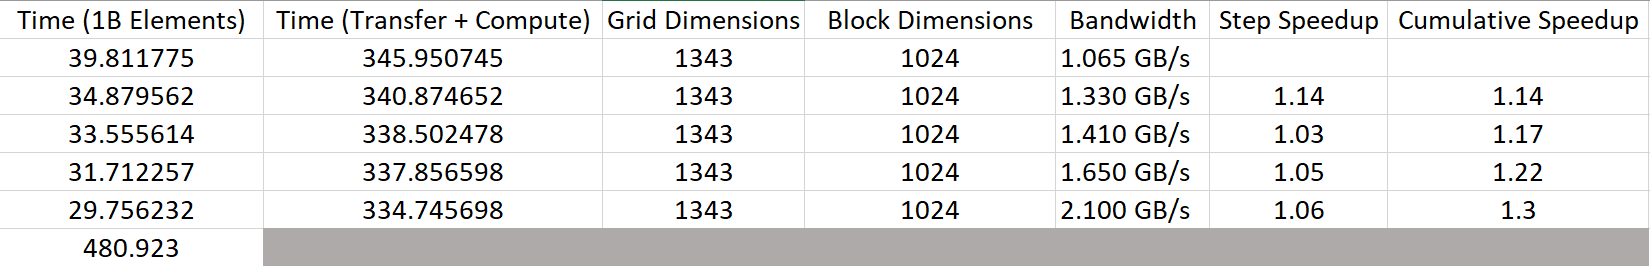
\includegraphics[width=1\textwidth]{speeds.png}
	\caption{Illustration of Serial \& Parallel Timings.}
	\label{pl1}
\end{figure}
\end{document}

